\sectionframe{Original Model}
\section{OG}

\begin{frame}{Model Origin}
	\begin{itemize}
		\item DC/AC power converter
		\item The converter switches $\Rightarrow$ models are piecewise-smooth and discontinuous
            \pause \vspace{1em}
		\item We focus on the time-discrete model
		\item It maps phase of the last switch $\theta_n$ to the phase of the next switch $\theta_{n+1}$
	\end{itemize}
\end{frame}

\begin{frame}{Model Definition (1/2)}
	\vspace{-2.0em}
	\begin{align}
		\theta_{n+1} & =  F(\theta_n) \mod 2 \pi
		\\
		F(\theta)    & = \begin{cases}
			                 F_1(\theta) & \text{if } q \cdot \cos(\theta) > 0 \\
			                 F_2(\theta) & \text{if } q \cdot \cos(\theta) < 0
		                 \end{cases}
		\\
		F_1(\theta)  & = \begin{cases}
			                 \theta + z_{L_+} + z_1 & \text{if } z_{L_+} < z_{L_0} \\
			                 \theta + z_{L_0} + z_2 & \text{if } z_{L_+} > z_{L_0}
		                 \end{cases}
		\\
		F_2(\theta)  & = \begin{cases}
			                 \theta + z_{R_+} + z_3 & \text{if } z_{R_+} < z_{R_0} \\
			                 \theta + z_{R_0} + z_4 & \text{if } z_{R_+} > z_{R_0}
		                 \end{cases}
	\end{align}

	\pause
	\vspace{2em}
	This looks ok, but how are these values defined?
	\begin{align*}
		z_1, z_2, z_3, z_4, z_{L_+}, z_{L_-}, z_{R_+}, \text{ and } z_{R_0}
	\end{align*}
\end{frame}

\begin{frame}{Model Definition (2/2)}
	\vspace{-1em}
	The smallest non-negative solutions to the following implicit equations
	\begin{subequations}
		\begin{align}
			(q \cdot \cos(\theta) + \mu \cdot \chi) \cdot e^{\lambda \cdot z_{L_+}}
			 & = q \cdot \cos(\theta + z_{L_+}) + \chi \label{equ:setup.og.def.impl.1.A}                  \\
			(q \cdot \cos(\theta) + \mu \cdot \chi) \cdot e^{\lambda \cdot z_{L_0}}
			 & = q \cdot \cos(\theta + z_{L_0}) - \chi                                                    \\
			(q \cdot \cos(\theta) - \mu \cdot \chi) \cdot e^{\lambda \cdot z_{R_+}}
			 & = q \cdot \cos(\theta + z_{R_+}) - \chi                                                    \\
			(q \cdot \cos(\theta) - \mu \cdot \chi) \cdot e^{\lambda \cdot z_{R_0}}
			 & = q \cdot \cos(\theta + z_{R_0}) + \chi \label{equ:setup.og.def.impl.1.D}
			\\
			(q \cdot \cos(\theta + z_{L_+}) + \chi + 1) \cdot e^{\lambda \cdot z_1} - 1
			 & = q \cdot  \cos(\theta + z_{L_+} + z_1) + \mu \cdot \chi \label{equ:setup.og.def.impl.2.A} \\
			(q \cdot \cos(\theta + z_{L_0} + z_2) - \chi - 1) \cdot e^{\lambda \cdot z_2} + 1
			 & = q \cdot  \cos(\theta + z_{L_0} + z_2) - \mu \cdot \chi                                   \\
			(q \cdot \cos(\theta + z_{R_+}) + \chi + 1) \cdot e^{\lambda \cdot z_3} - 1
			 & = q \cdot  \cos(\theta + z_{L_+} + z_1) + \mu \cdot \chi                                   \\
			(q \cdot \cos(\theta + z_{R_0} + z_4) - \chi - 1) \cdot e^{\lambda \cdot z_4} + 1
			 & = q \cdot  \cos(\theta + z_{R_0} + z_2) - \mu \cdot \chi \label{equ:setup.og.def.impl.2.D}
		\end{align}
	\end{subequations}
	\begin{flushright}
		Definition from \cite{akyuz2022}
	\end{flushright}
\end{frame}

\begin{frame}{Unusual Bifurcation Structure}
	\begin{figure}
		\only<1>{
			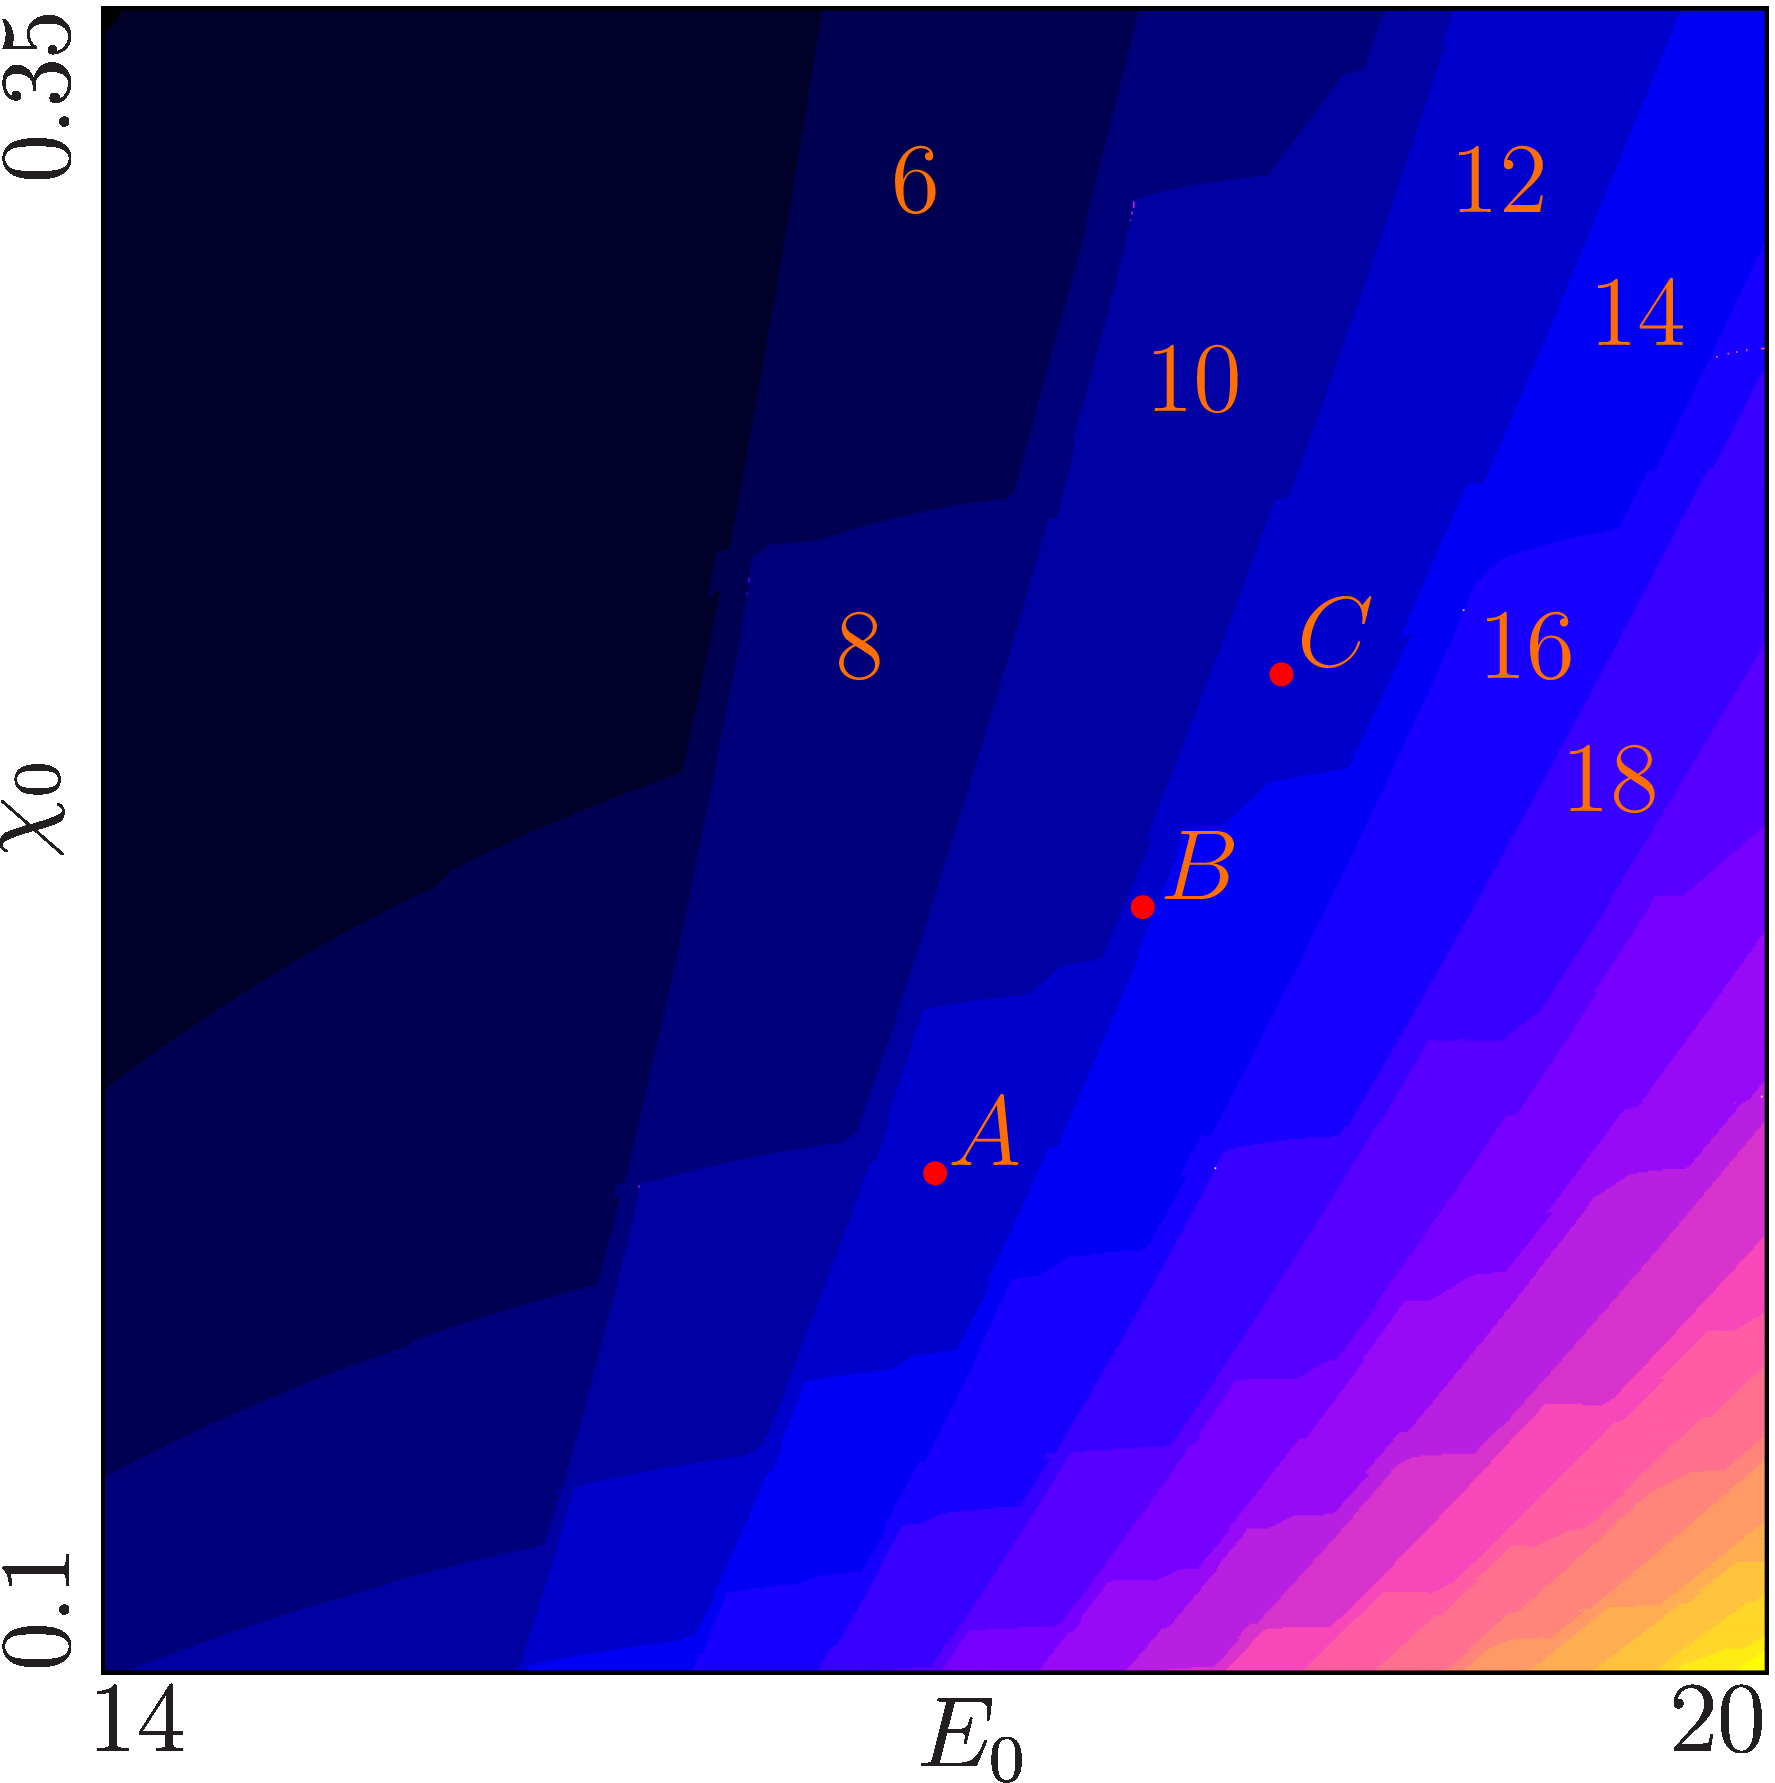
\includegraphics[width=0.45 \textwidth]{../Figures/2/2.3/result.png}
		}
		\only<2>{
			\stackunder[5pt]{
				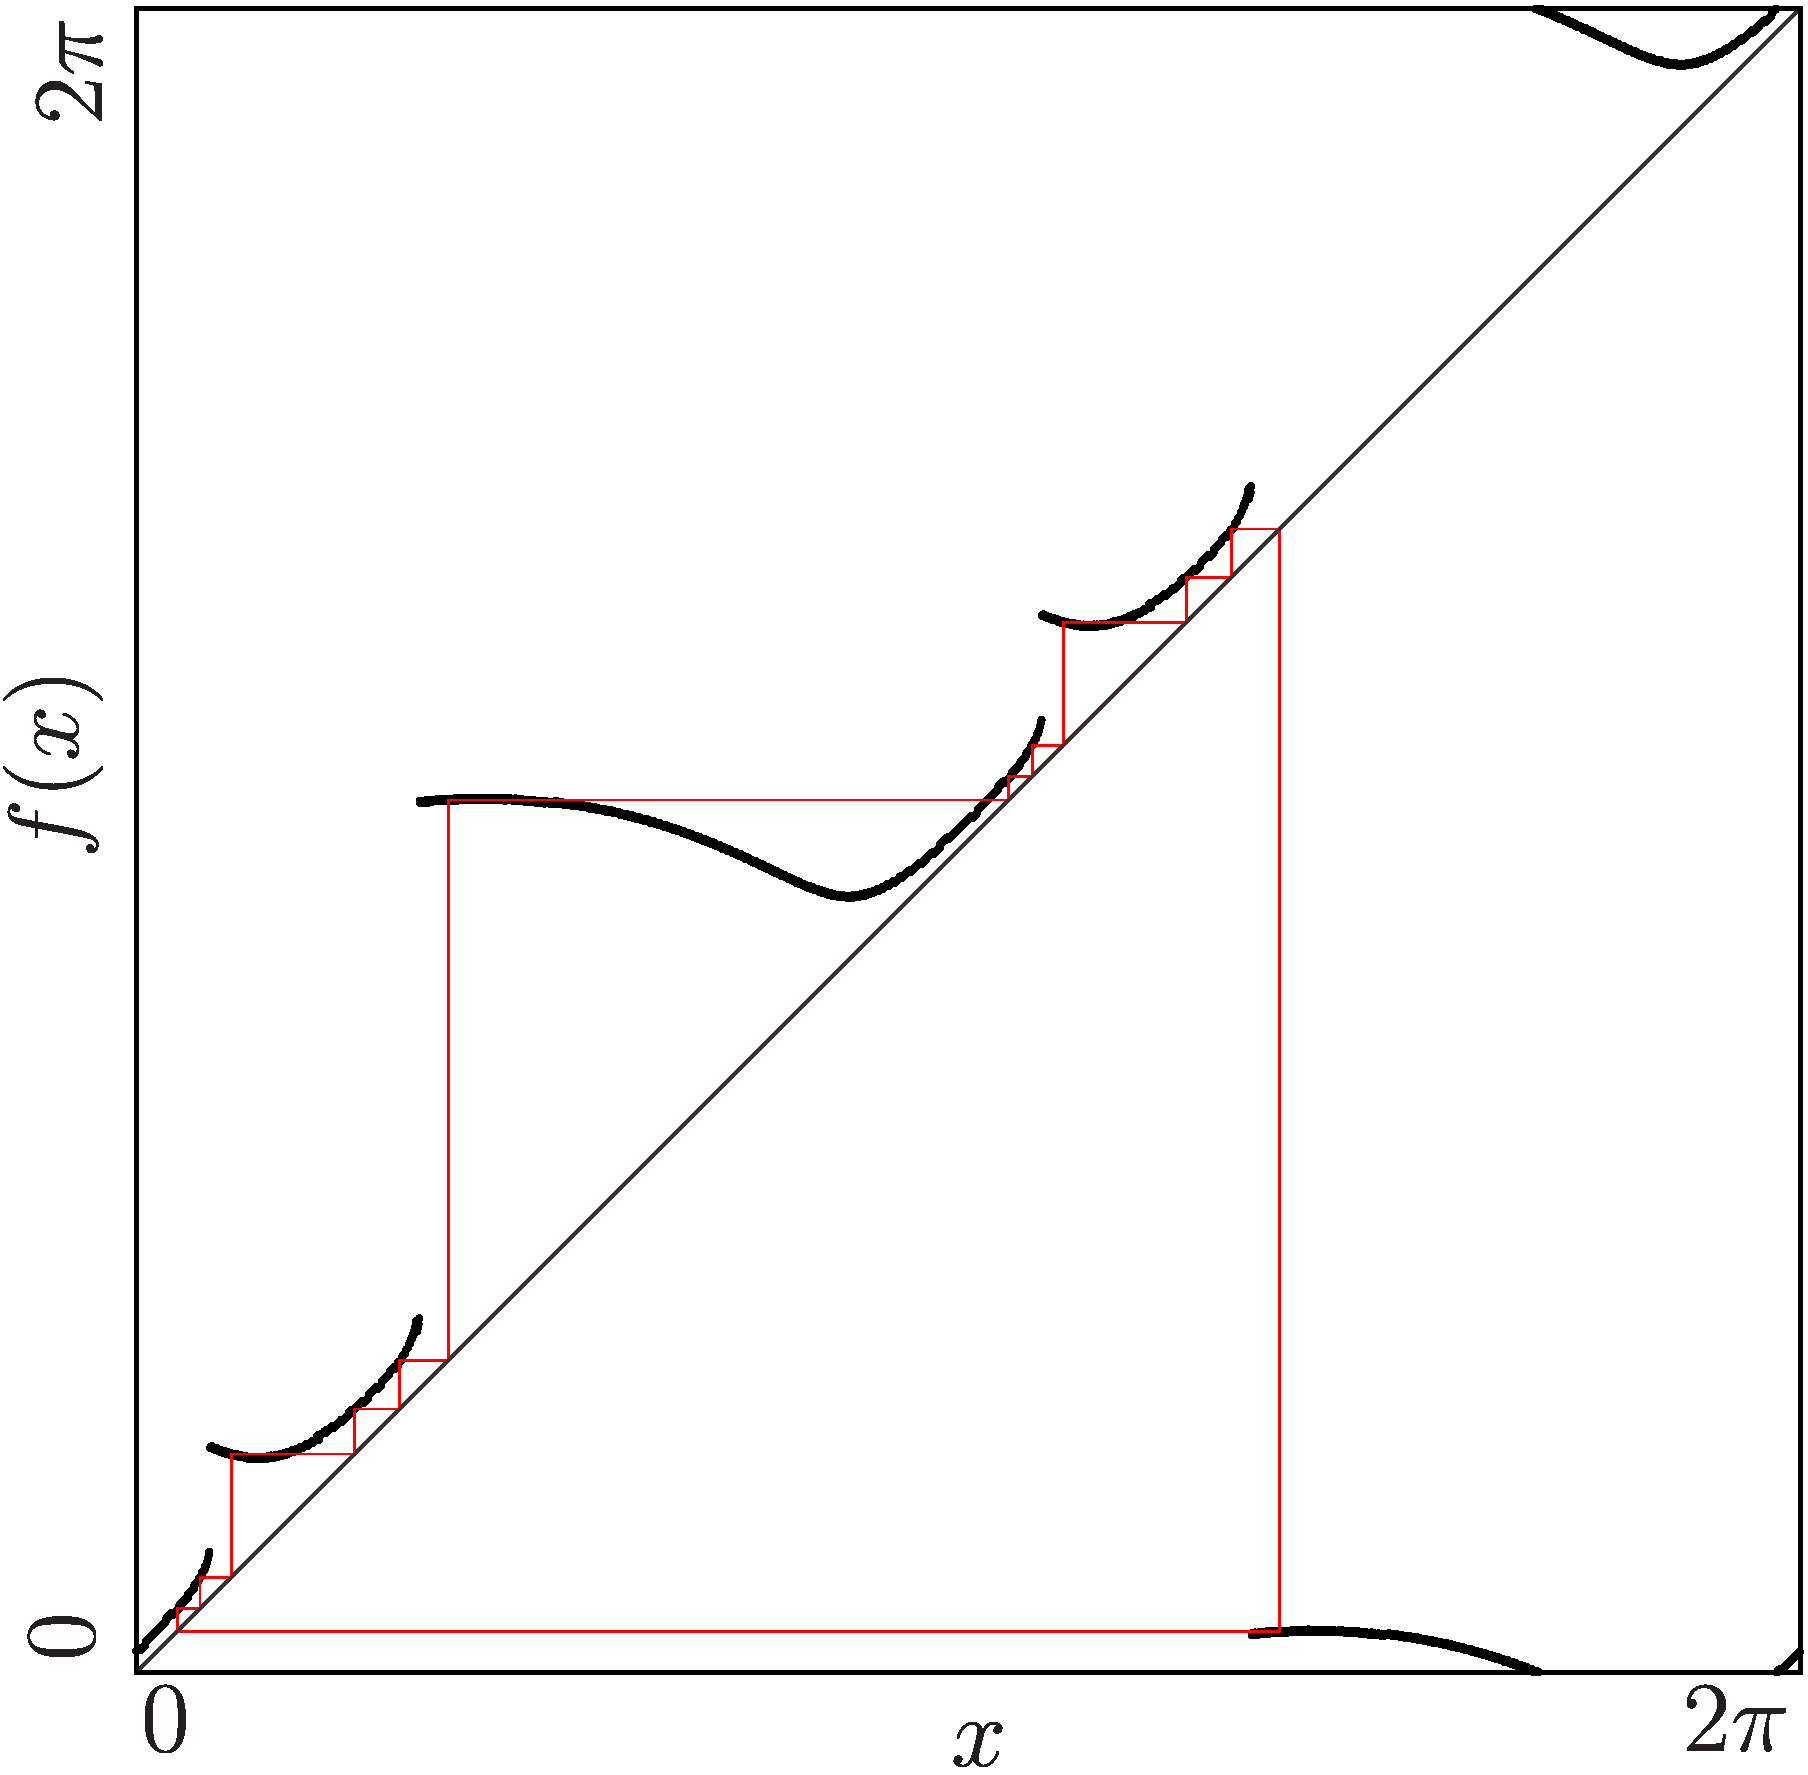
\includegraphics[width=0.3 \textwidth]{../Figures/2/2.4a/result.png}
			}{$A:\:\A^3\B^3\C^3\D^3$}
			\stackunder[5pt]{
				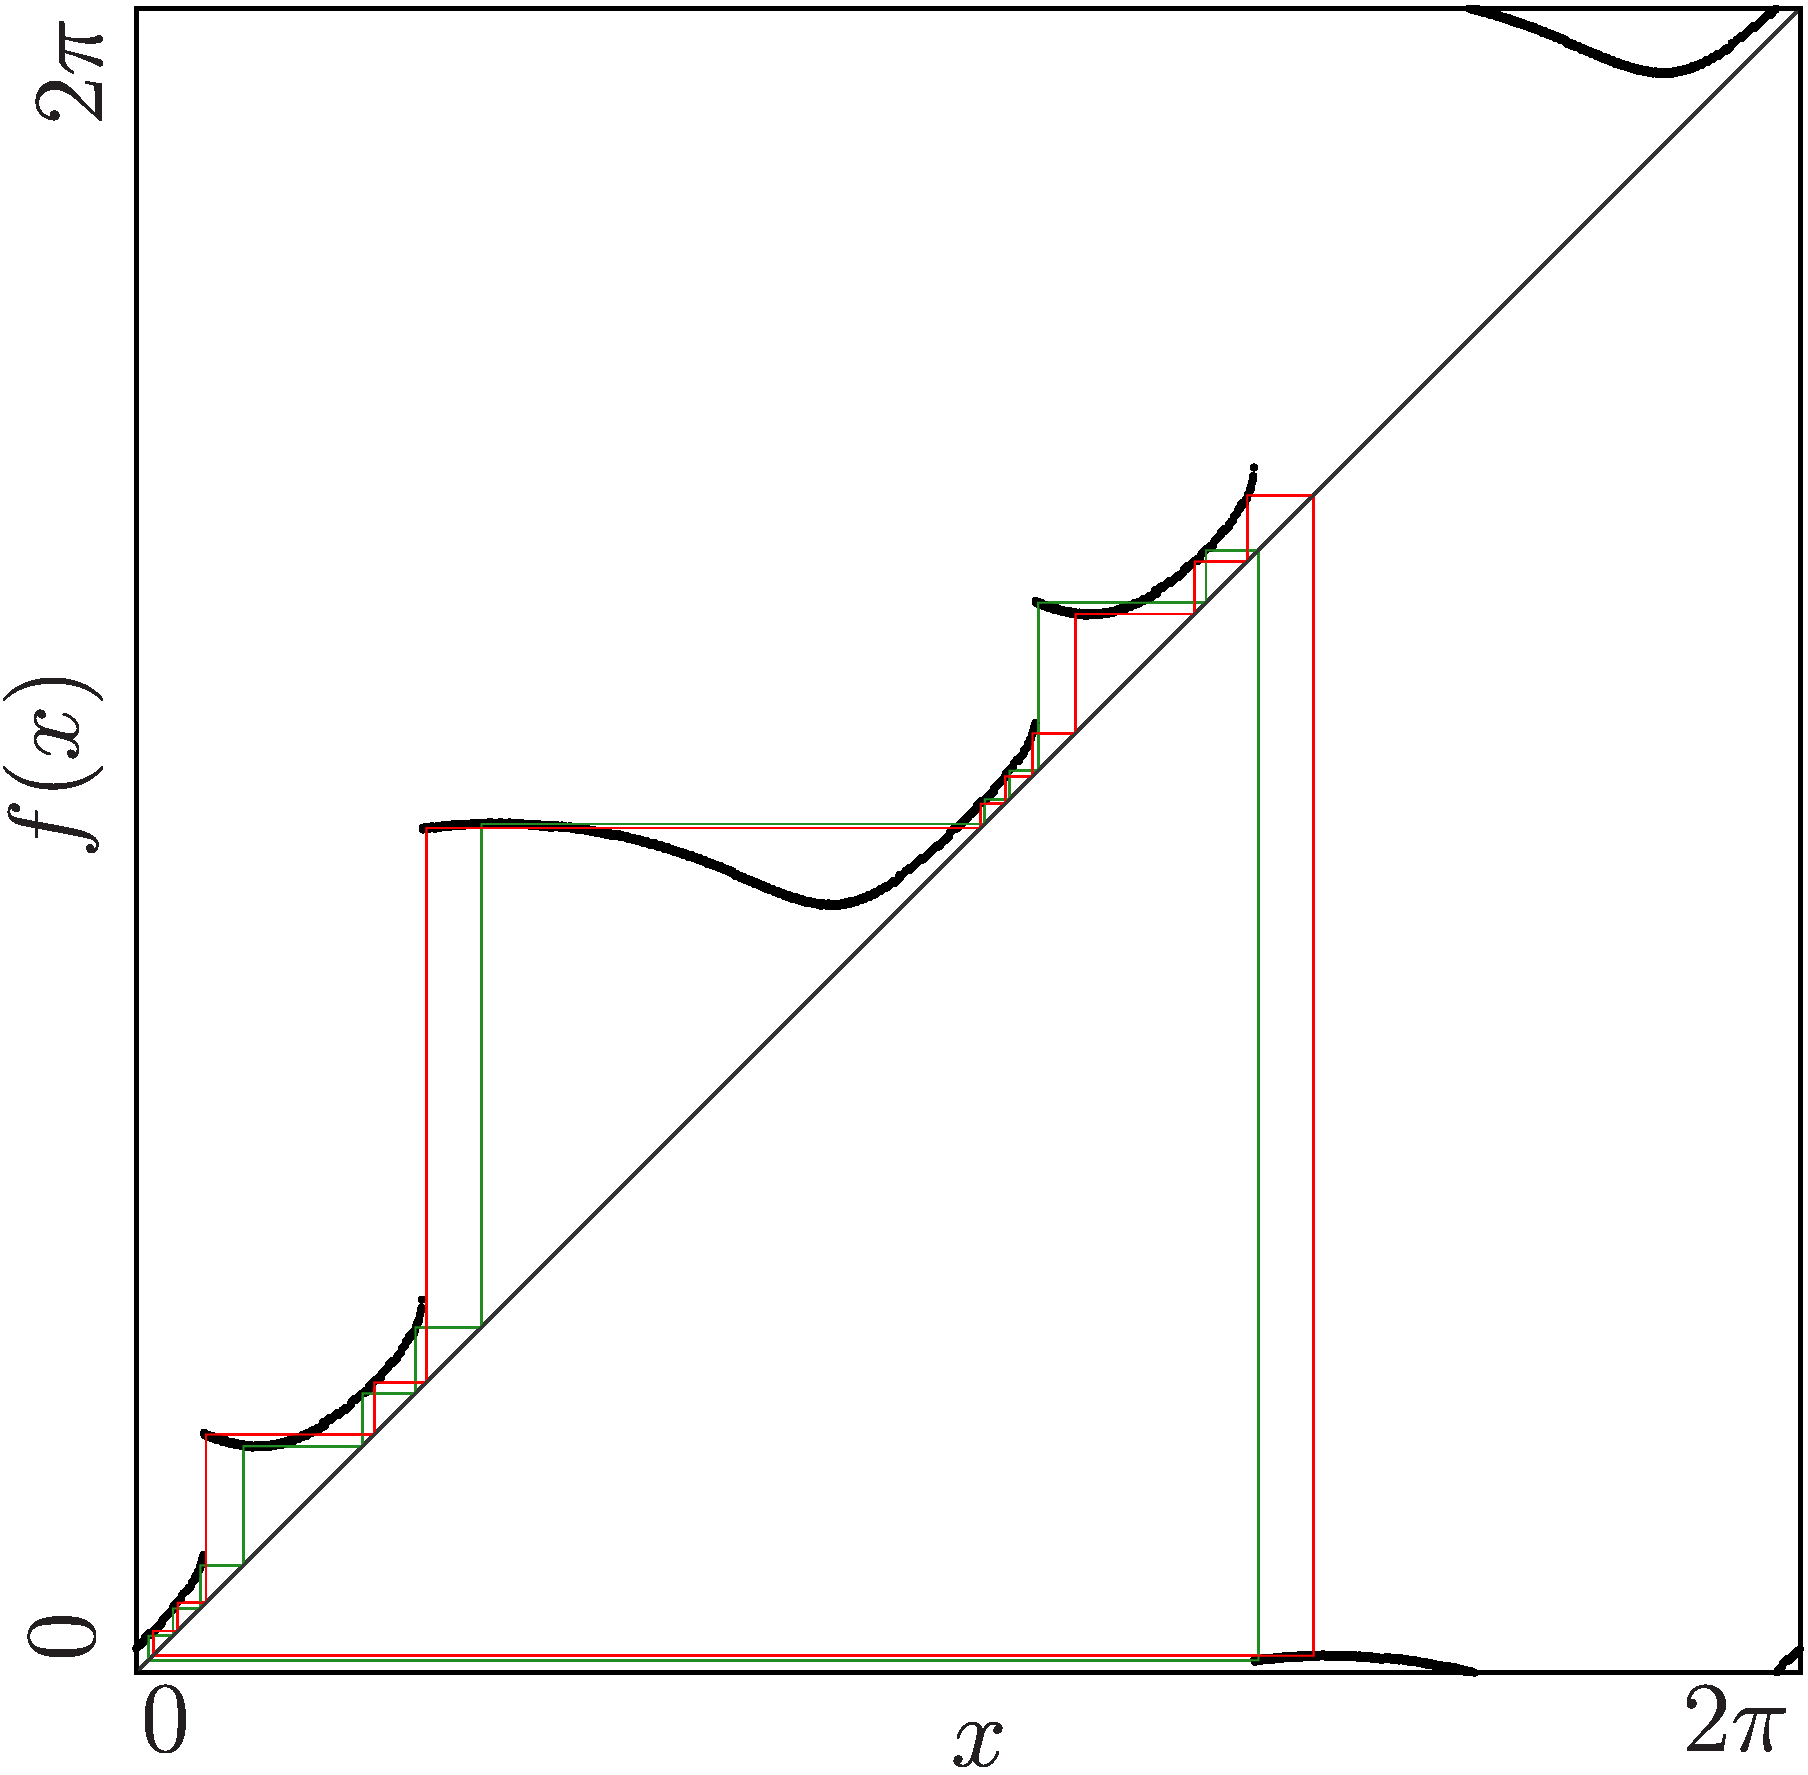
\includegraphics[width=0.3 \textwidth]{../Figures/2/2.4b/result.png}
			}{$B:\:\A^3\B^3\C^2\D^4,\:\A^2\B^4\C^3\D^3$}
			\stackunder[5pt]{
				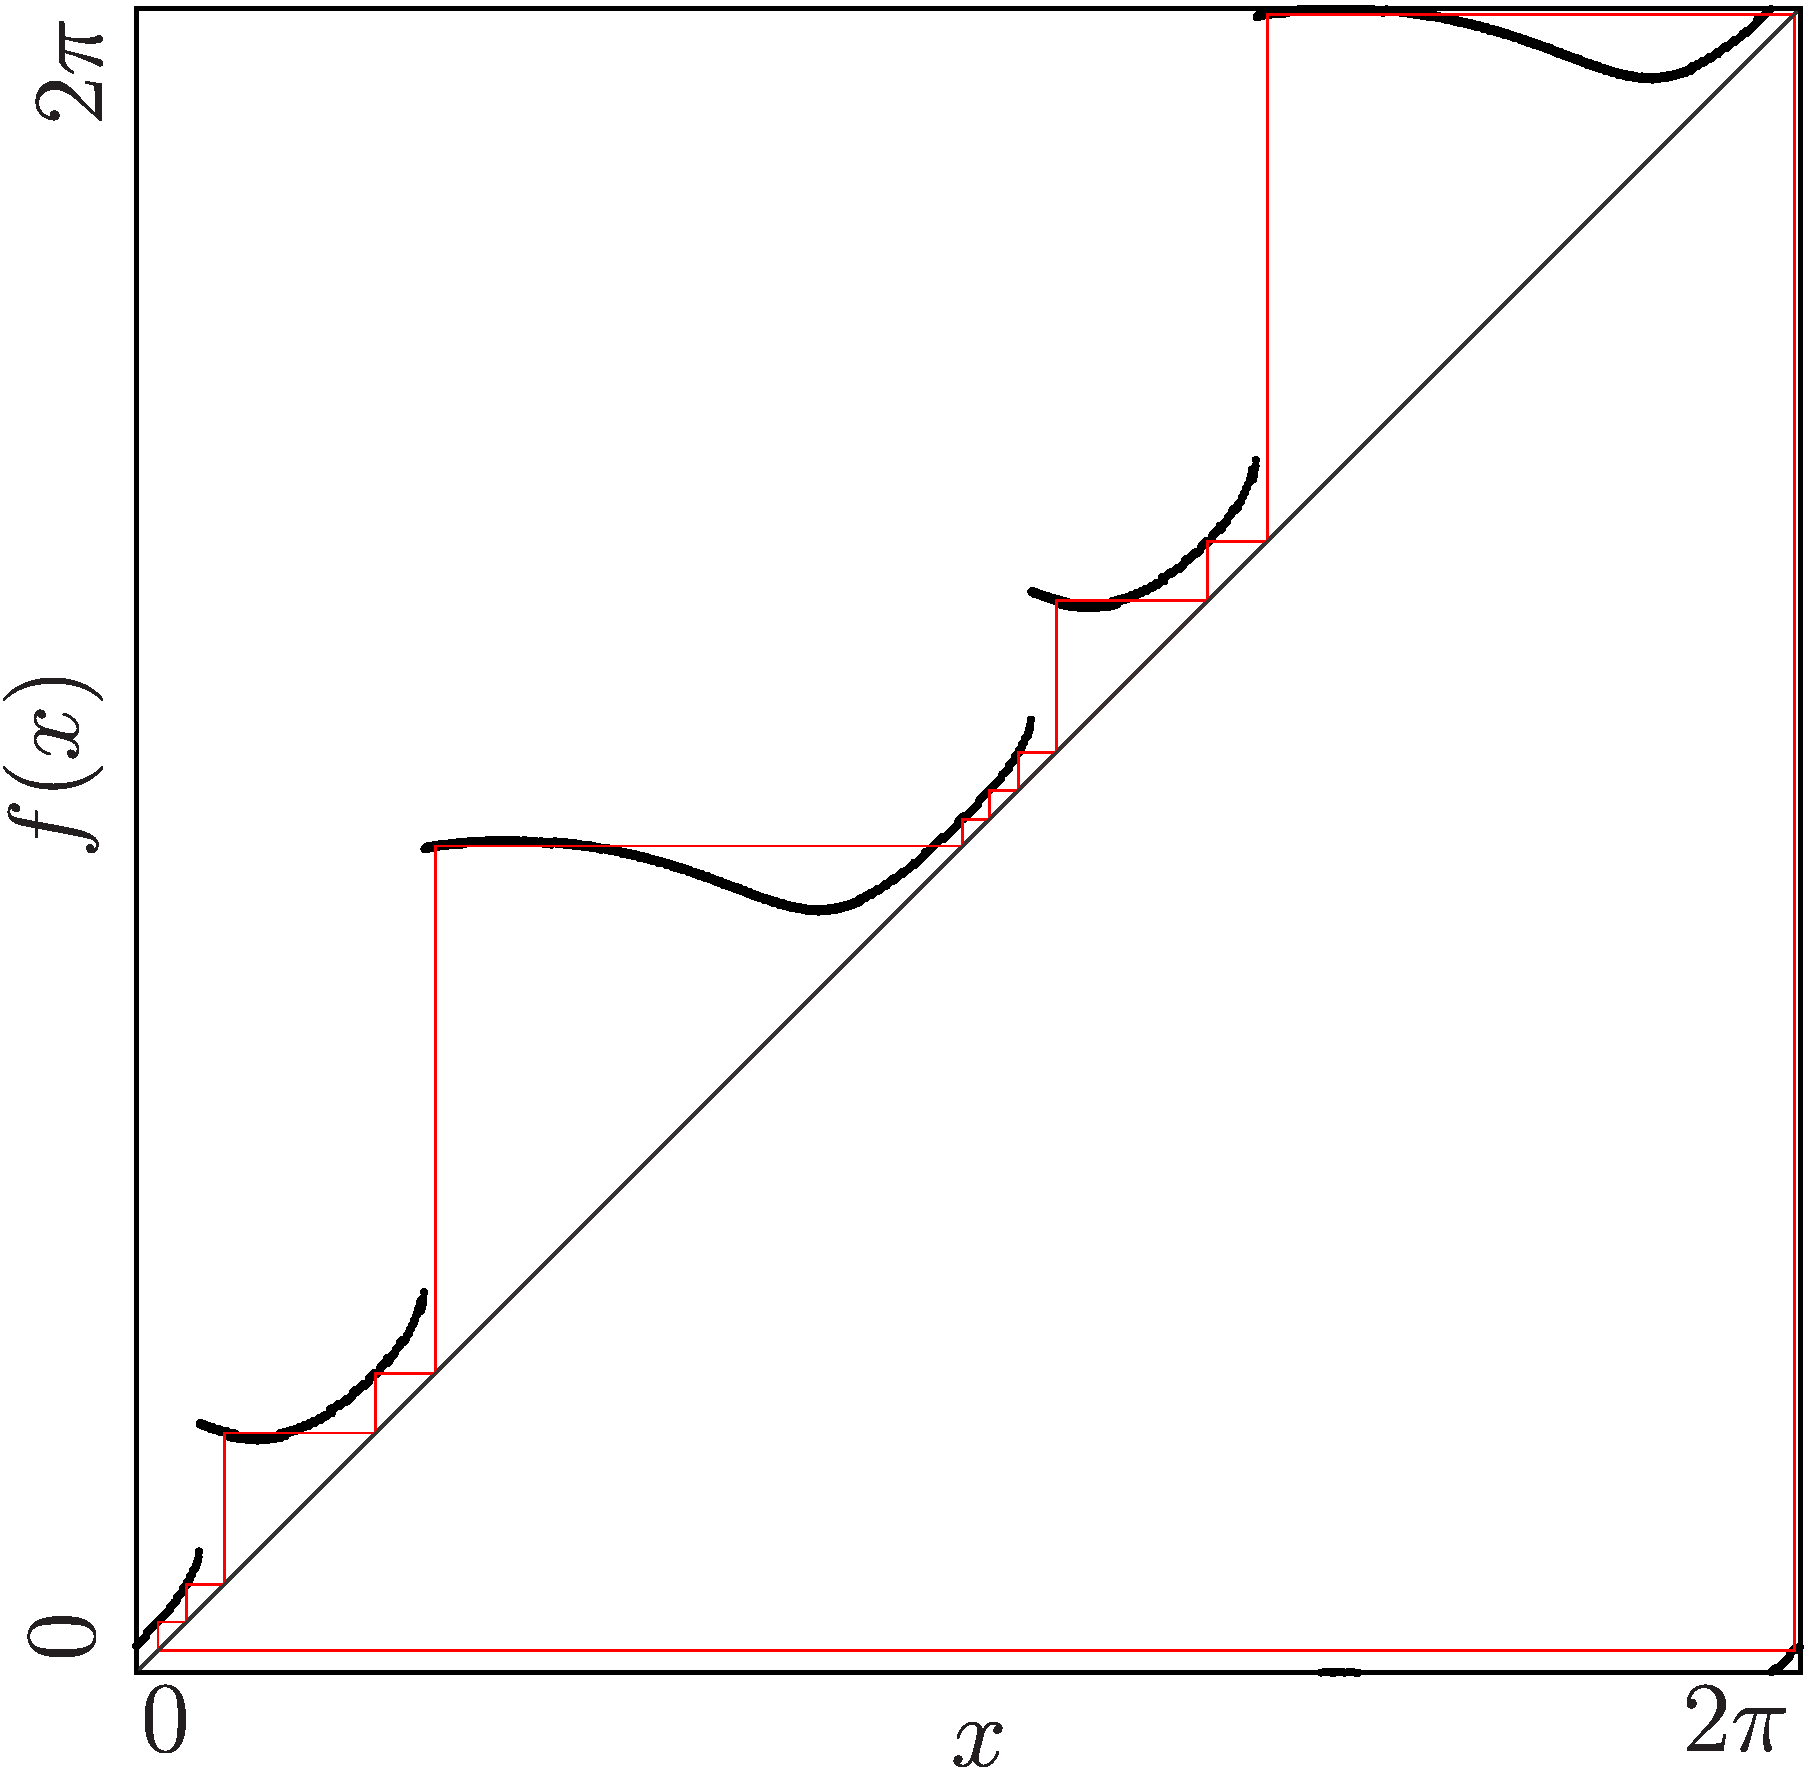
\includegraphics[width=0.3 \textwidth]{../Figures/2/2.4c/result.png}
			}{$C:\:\A^2\B^4\C^2\D^4$}
		}
	\end{figure}
	\pause
	\vspace{1em}
	Symmetry $F(\theta + \pi) = F(\theta) + \pi \mod 2\pi$ \hfill \cite{akyuz2022}
\end{frame}
